%!TEX root = P231_notes.tex

\section{The Harmonic Oscillator}
% \lecdate{lec~12}

Let's return to the problem of solving for Green's functions. Let's focus on our favorite example---arguably, the \emph{only} example\footnote{Upon generalizing to higher dimensions, curvilinear coordinates. Physicists have Harmonic Oscillators in different area codes.}---is the harmonic oscillator. The differential operator is
\begin{align}
	\mathcal O = \left(\frac{d}{dt}\right)^2 + \omega_0^2 \ .
	\label{eq:O:HO}
\end{align}
The Green's function equation tells us the response $G(t,t_0)$ at time $t$ from a `unit displacement' at $t_0$:
\begin{align}
	G''(t,t_0) + \omega_0^2 G(t,t_0) = \delta(t-t_0) \ .
	\label{eq:HO:Greens:eqn}
\end{align}
Recall that the arguments $t$ and $t_0$ are analogous to the indices of a finite-dimensional matrix. For notational convenience, we will set $t_0=0$ and not list it explicitly. We are primarily concerned about the $t$-dependence of $G(t,t_0)$. 

\subsection{Fourier Transform}

The first thing we're going to do is write $G(t,t_0)$ as a Fourier transform with respect to $t$. Please refer to Appendix~\ref{app:Fourier} for our set of Fourier transform conventions. We can write $G(t)$ as an integral over Fourier modes with frequency $\omega$ and weight (Fourier transform) $\tilde G(\omega)$:
\begin{align}
	G(t) &= \int_{-\infty}^\infty\dbar \omega \, e^{-i\omega t} \tilde G(\omega) 
	&
	\dbar = \frac{d}{2\pi}
	\ .
	\label{eq:HO:Greens:Fourier}
\end{align}
We say that $\tilde G(\omega)$ is the Fourier transform of $G(t)$. The key point is that the $t$-dependence of $G(t)$ has been sequestered into the $e^{-i\omega t}$ plane waves. This is convenient since these plane waves are eigenfunctions of the derivative operator:
\begin{align}
	\frac{d}{dt} e^{-i\omega t} &= -i\omega e^{-i\omega t} \ .
\end{align}
The left-hand side of the Green's function equation \eqref{eq:HO:Greens:eqn} is
\begin{align}
	\mathcal O_t G(t,t_0) 
	&= 
	-
	\int_{-\infty}^\infty \dbar \omega \, 
	\left(\omega^2-\omega_0^2\right) e^{-i\omega t} \tilde G(\omega,t_0) \ .
\end{align}
The right-hand side is simply the Fourier transform of $\delta(t-t_0)$:
\begin{align}
	\delta(t-t_0)
	&=
	\int_{-\infty}^\infty \dbar \omega \, e^{-i\omega (t-t_0)} \ .
	\label{eq:delta:fourier}
\end{align}
\begin{exercise}
Use our conventions for the Fourier transform \eqref{eq:HO:Greens:Fourier} (see also Appendix~\ref{app:Fourier}) to confirm the Fourier representation of $\delta(t-t_0)$ in \eqref{eq:delta:fourier}. In our notation, the Fourier coefficients $\tilde f(\omega)$ of a function $f(t)$ is
\begin{align}
	\tilde f(\omega) &= 
	% \frac{1}{2\pi}
	\int_{-\infty}^\infty d t\, e^{i\omega t} f(t) \ .
\end{align}
\end{exercise}
So the Green's function equation for the 1D harmonic oscillator, \eqref{eq:HO:Greens:eqn}, tells us
\begin{align}
	-
	\int_{-\infty}^\infty \dbar \omega \, 
	\left(\omega^2-\omega_0^2\right) e^{-i\omega t} \tilde G(\omega)
	&=
	\int_{-\infty}^\infty \dbar \omega \, e^{i\omega t}
	\ .
	\label{eq:G:HO:Fourier:equation:integrals}
\end{align}
For simplicity we have set $t_0=0$ and don't write it explicitly. There's a rather unscrupulous\footnote{I don't think this is rigorously valid, but the result is true. The ends don't justify the means, but let's take this morally ambiguous shortcut to make the big picture clear. I encourage you to live the rest of your lives with virtue.} way to solve this equation for $\tilde G(\omega)$. Since the two sides of this expression are equal, they have the same Fourier expansion. This implies that the Fourier coefficients are equal. Since both sides are already written as Fourier expansions, we can just match the coefficients of the basis functions, $e^{-i\omega t}$. This gives us:
\begin{align}
	\tilde G(\omega) &= \frac{-1}{\omega^2-\omega_0^2}
	\label{eq:G:HO:Fourier:term}
\end{align}
\begin{exercise}
Prove \eqref{eq:G:HO:Fourier:term} honestly. {Hint}: Start with \eqref{eq:G:HO:Fourier:equation:integrals} and project out the Fourier coefficients. Recall that you do this by taking the inner product with one of the basis functions and then using the orthogonality of the eigenbasis. You may need to be careful with the normalization.
\end{exercise}
\begin{exercise}
In \eqref{eq:G:HO:Fourier:equation:integrals} we had already set $t_0 = 0$. What is the expression for $\tilde G(\omega)$ if we kept $t_0$ explicit?
\label{eq:ex:Gtilde:with:t0:explicit}
\end{exercise}
That was the critical step: we have successfully solved for the Green's function Fourier coefficient. This means that we have a closed form expression for the Green's function by plugging $\tilde G(\omega)$ into \eqref{eq:HO:Greens:Fourier}:
\begin{align}
	G(t) &=  \int_{-\infty}^\infty \dbar \omega
	\, 
	\frac{-e^{-i\omega t}}{\omega^2-\omega_0^2} \ .
	\label{eq:G:HO:Fourier:Rep:t0:0}
\end{align}
All that's left is for us to actually \emph{do} this integral. Fortunately, this integral should look very similar. It seems to beg for us to solve using the residue theorem. 
\begin{exercise}
What are the poles of the integrand in \eqref{eq:G:HO:Fourier:Rep:t0:0}? What are their associated residues? What is the residue if $t_0\neq 0$?
\end{exercise}

\subsection{Contour Integral}

The integral \eqref{eq:G:HO:Fourier:Rep:t0:0} looks like it's perfect for contour integration. There's an exponential factor on top that will determine the convergence, and the denominator can be factored to see where the poles are. Except we notice something troubling:
\begin{align}
	\frac{-e^{-i\omega t}}{\omega^2-\omega_0^2} 
	&=
	\frac{-e^{-i\omega t}}{(\omega - \omega_0)(\omega + \omega_0)} \ .
	\label{eq:HO:integrand:real:pole}
\end{align}
The poles are located at $\omega = \pm \omega_0$. These are \emph{on the real axis}, precisely along the integration contour! How annoying!

Now you may want to have an existential moment. Remind yourself that all we're doing is solving for the behavior of the one-dimensional \emph{harmonic oscillator}. This is an eminently \emph{physical} system. We could have written this system as $\mathcal O f(t) = s(t)$ where $f(t)$ is the displacement of a harmonic oscillator and $s(t)$ is some driving function. The Green's function, $G(t,t_0)$ gives the response of the system to a `unit' driving function, $s(t) = \delta(t-t_0)$. The response of the system should be perfectly physical. And yet---\emph{and yet}---we now face an integral \eqref{eq:G:HO:Fourier:Rep:t0:0} that seems to run right into not only one, but \emph{two} singularities along the integration contour!
\begin{center}
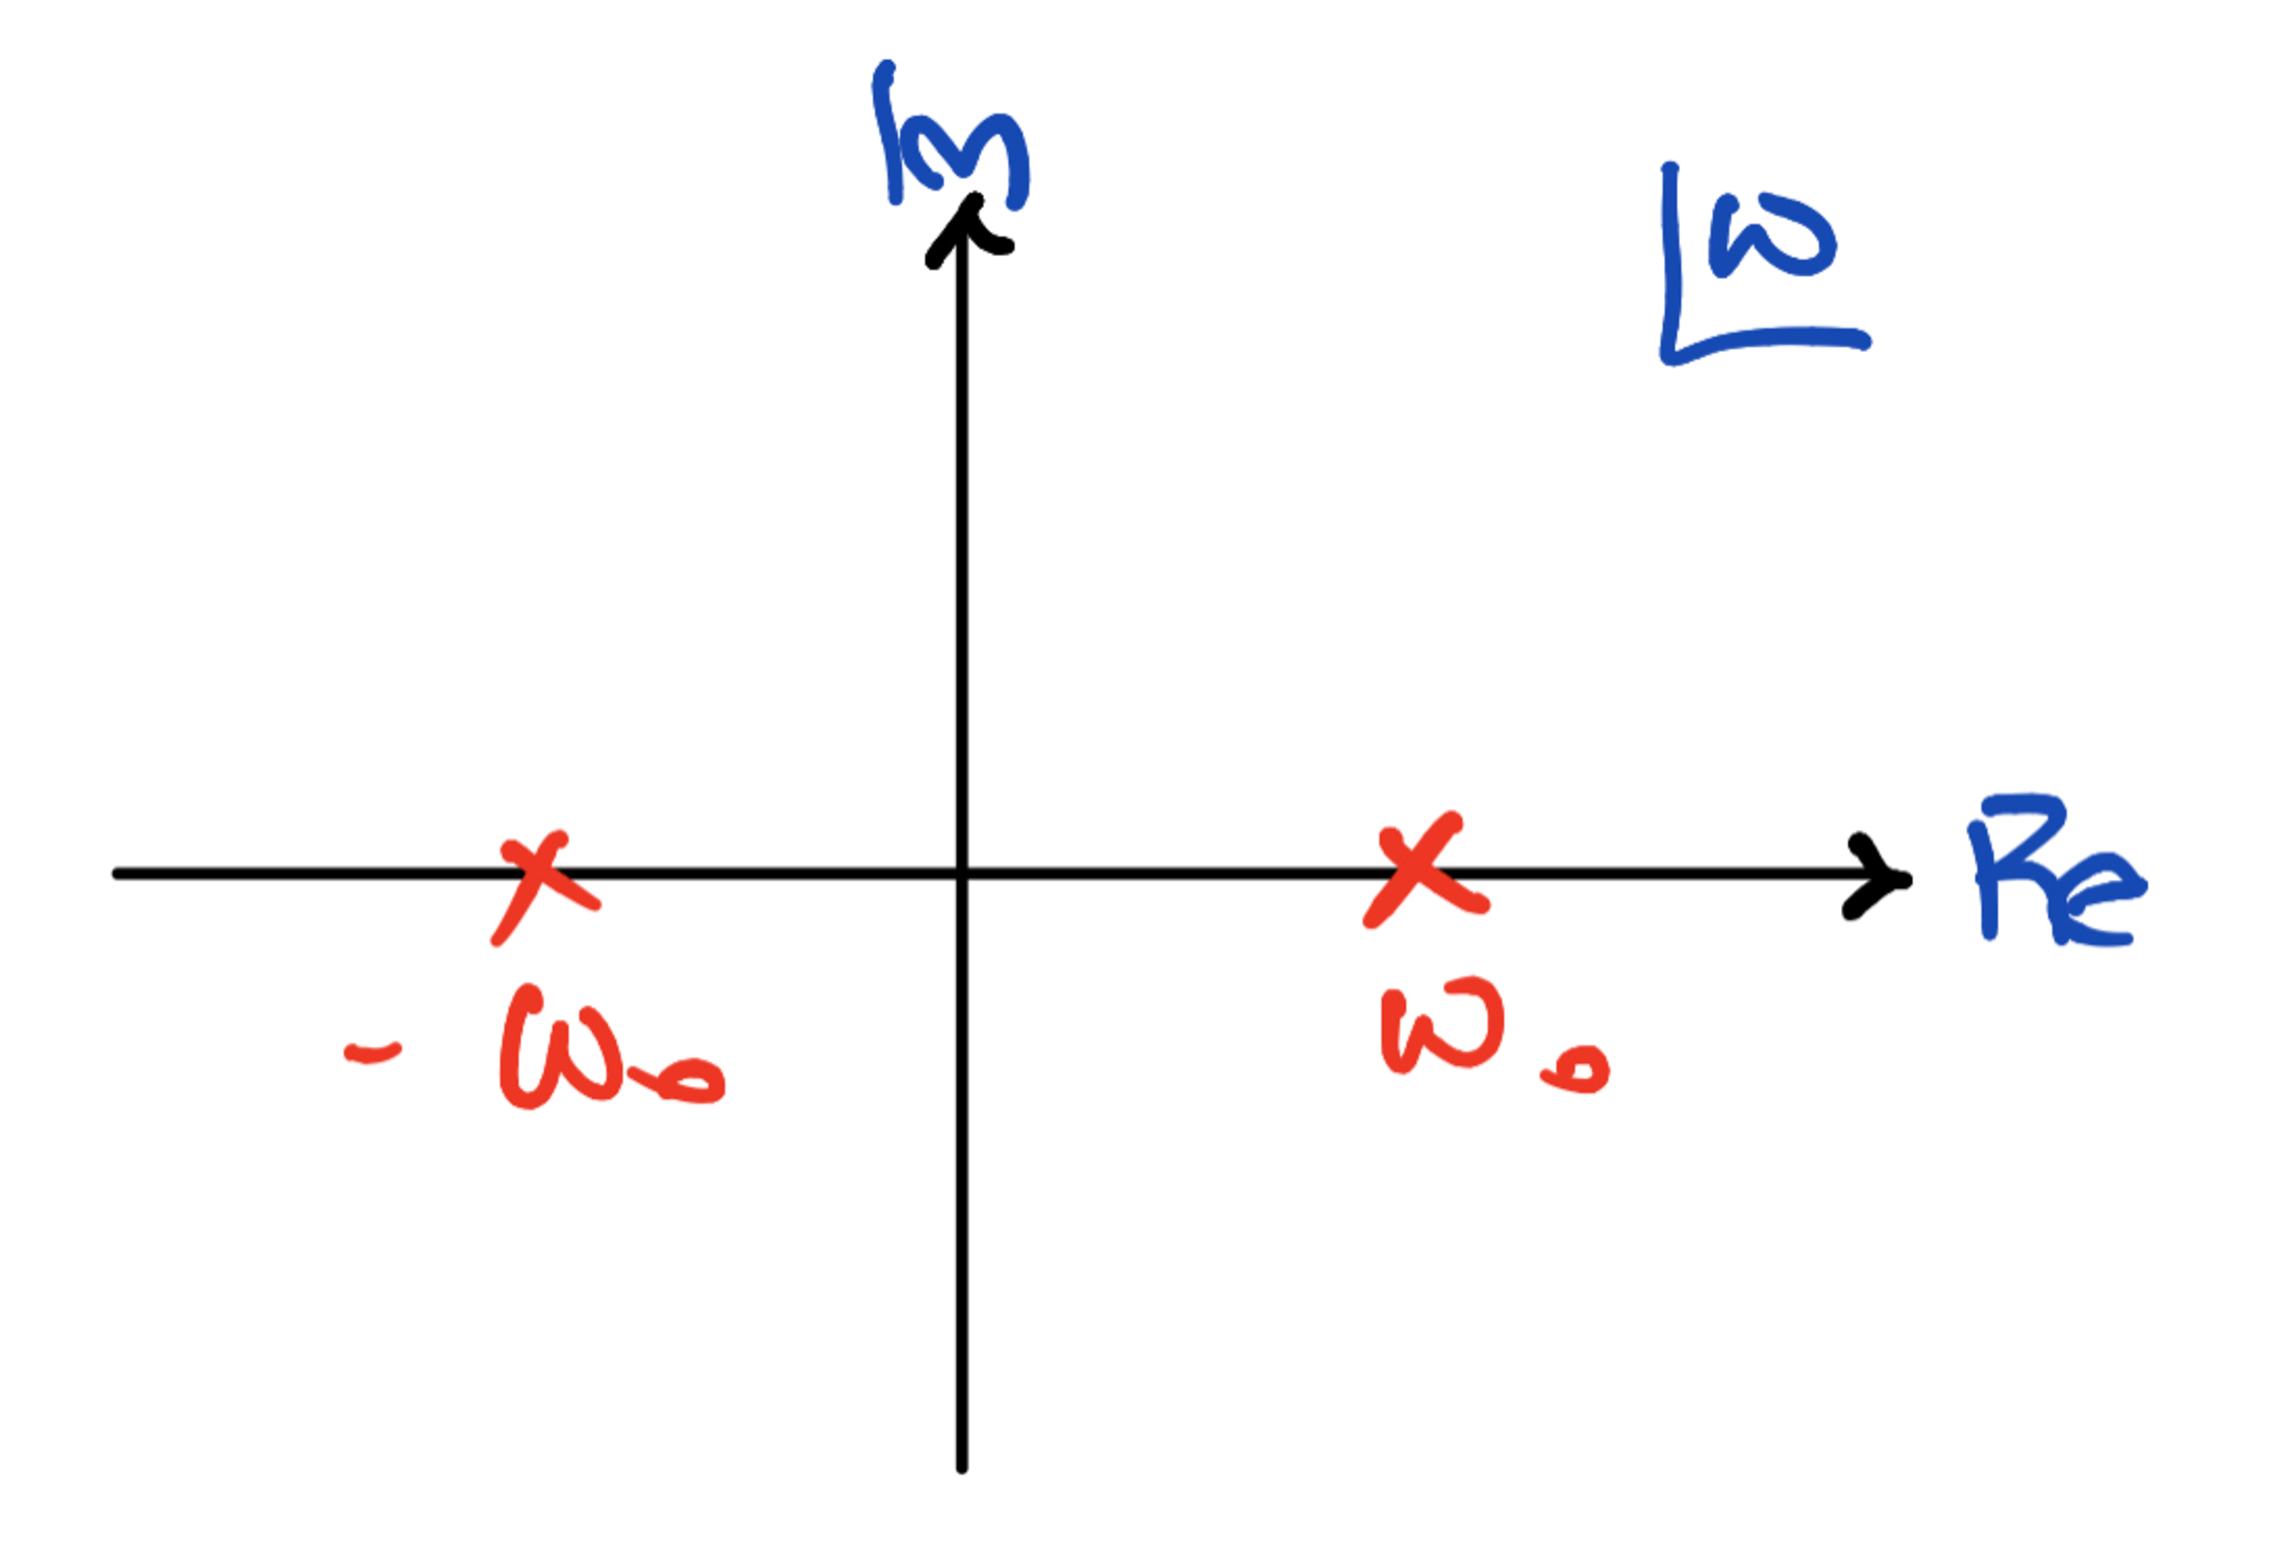
\includegraphics[width=.4\textwidth]{figures/Lec_2017_16_HO_Poles.pdf}
\end{center}
Please do take a brief moment to ponder at this existential crisis. This is an apparent failure of our theory---our calculation hits a pole, you get an infinity, and it's not clear what's going on. Rather than anguish, though, we should see if our theory is trying to tell us something. 

In order to figure out what's going on, let's do something wild. The poles on the real axis are in the way. Let's just move them out of the way by giving them small imaginary parts\footnote{I have altered the poles. Pray that I do not alter them further.}. Each pole can either be pushed above or below the real line:
\begin{center}
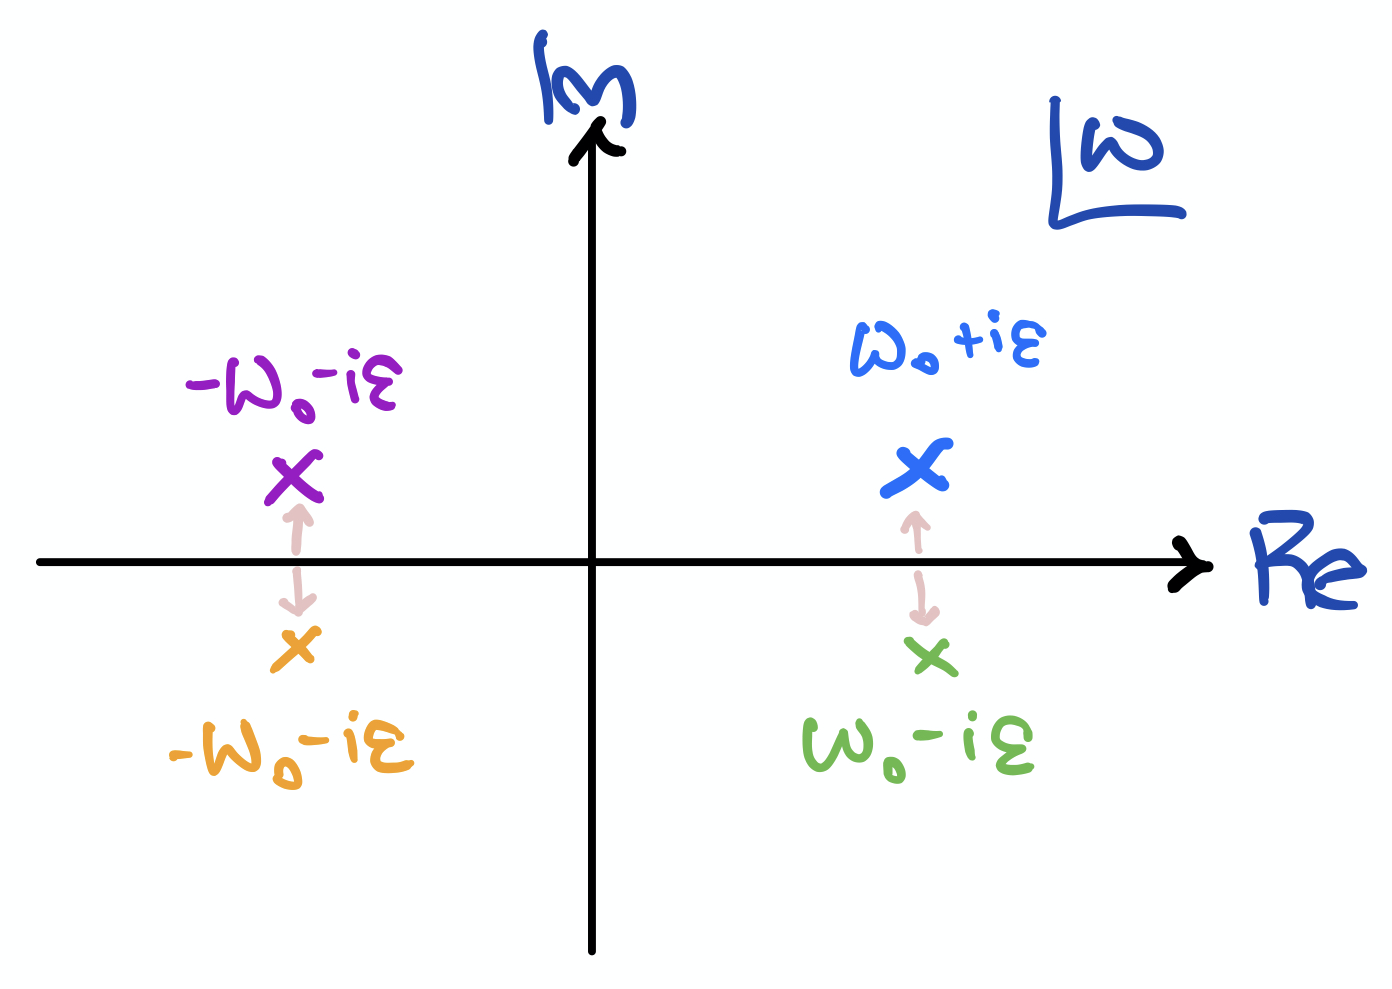
\includegraphics[width=.4\textwidth]{figures/Lec_2017_16_HO_PoleShift.png}
\end{center}
To be clear: are \emph{changing} the integral. We are exploring what happens when the expression \eqref{eq:G:HO:Fourier:Rep:t0:0} is changed, as if the poles were slightly complex the whole time. In other words, we are \emph{changing} the original differential operator, \eqref{eq:O:HO}. We're not yet motivating \emph{why} we want to do this; we'll justify it post-facto. For now, let's just be happy that our contours no longer bump into the poles. 

\subsection{Going under the poles?}
Let's try going under the poles, that is: let's push the poles into the upper half-plane with small imaginary parts:
\begin{center}
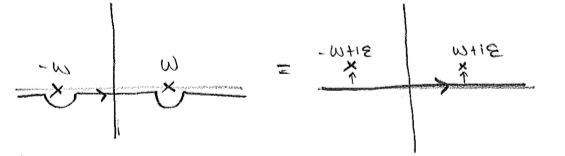
\includegraphics[width=.6\textwidth]{figures/Lec_2017_16_underpole.png}
\end{center}
This means that we have deformed the integrand \eqref{eq:HO:integrand:real:pole}:
\begin{align}
\frac{-e^{-i\omega t}}{(\omega - \omega_0)(\omega + \omega_0)}
&\to
\frac{-e^{-i\omega t}}{(\omega - \omega_0 - i\varepsilon)(\omega + \omega_0 - i\varepsilon)} \ .
\label{eq:HO:integrand:upper:poles}
\end{align}
To make it clear that we are treating $\omega$ as a complexified variable, let's write it as $z$:
\begin{align}
 	\omega \to z \ .
 \end{align}
Now let's go through the exercise of performing the integral along the real line by using the residue theorem. To do this have to choose a contour that includes the real line. We have two options, $C_+$ and $\bar C_-$, where the bar reminds us of the orientation:
\begin{center}
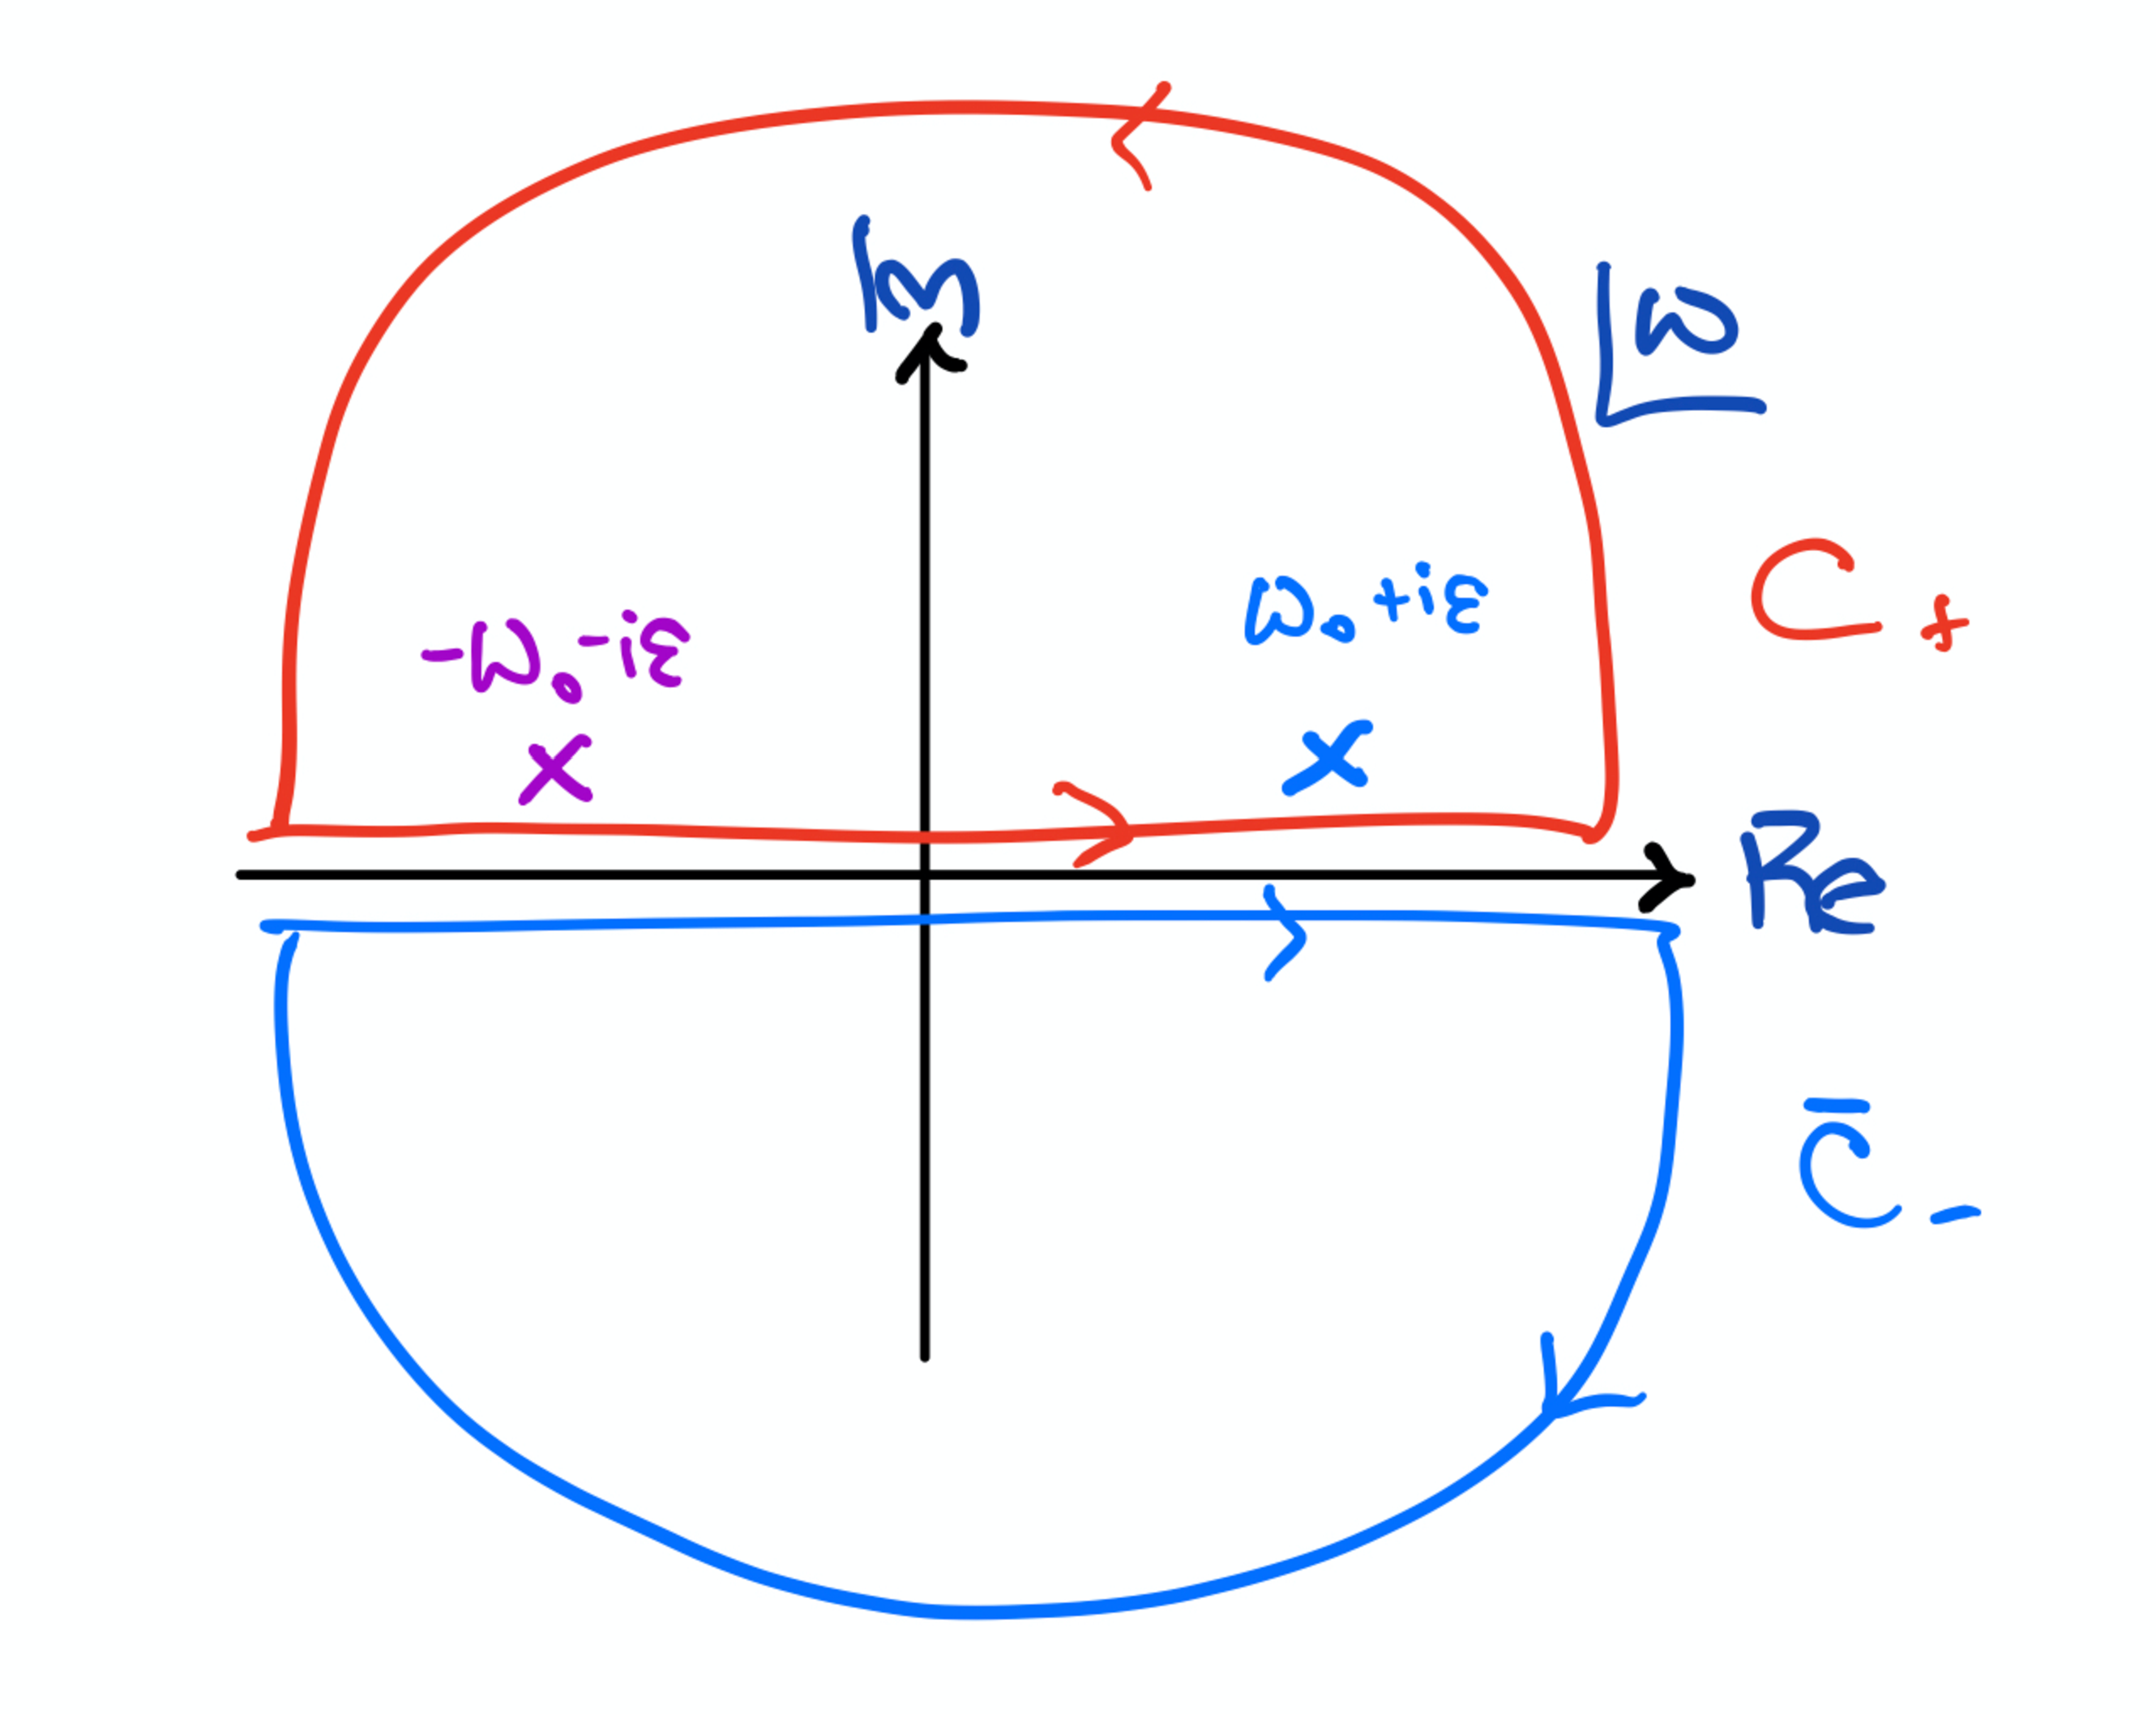
\includegraphics[width=.4\textwidth]{figures/Lec_2017_16_pokeup.pdf}
\end{center}
Which contour do we pick? Does it matter? (Yes!) The contours differ by whether the `large arc' has positive or negative real part. We can parameterize these arcs as we did in \eqref{eq:z:paramterization:large:arc}:
\begin{align}
	z(\theta) &= R\cos\theta + i R\sin\theta \ ,
\end{align}
where for $C_+$ the arc is given by $\theta \in [0,\pi]$ while for $\bar C_-$ the arc is $\theta\in[\pi,2\pi]$. In other words, 
\begin{align}
	\text{for $C_+$:}\, \sin\theta &> 0
	&
	\text{for $\bar C_-$:}\, \sin\theta &<0 \ .
	\label{eq:HO:which:contour}
\end{align}
%
How do we pick? The criteria for completing the real line into a contour is that the integral along the contour vanishes, that way
\begin{align}
	\oint_C dz\, f(z) 
	= \int_{-\infty}^\infty dx\, f(x) + \lim_{R\to \infty} R \int_\text{arc} d\theta f(Re^{i\theta}) 
	= \int_{-\infty}^\infty dx\, f(x) \ .
\end{align}
And hence one can use the residue theorem to solve the contour integral on the left-hand side and relate it to the real integral on the right-hand side\footnote{I say `real integral' but of course the integrand \eqref{eq:HO:integrand:upper:poles} is now a complex quantity, but the point is that we're only integrating along the real line.}. 
%
So which contour satisfies
\begin{align}
	\lim_{R\to \infty} R \int_\text{arc} d\theta 
	% f(Re^{i\theta})  
	\frac{-e^{-i(R\cos\theta + iR\sin\theta) t}}{(Re^{i\theta} - \omega_0 - i\varepsilon)(Re^{i\theta} + \omega_0 - i\varepsilon)}
	\to 0 \ ?
\end{align}
I was a little slick and chose to write $z = R\cos\theta + iR\sin\theta$ in the numerator while writing the more compact $z=Re^{i\theta}$ in the denominator. The convergence\footnote{I tend to say convergence, what I really mean is `vanishes as $R\to \infty$.'} of the integrand depends on the exponential factor in the numerator:
\begin{align}
	e^{-i(R\cos\theta + iR\sin\theta) t} = 
	e^{-iRt\cos\theta} e^{Rt\sin\theta} \ .
\end{align}
We can see that the convergence depends specifically on the second factor, $e^{-Rt\sin\theta}$. Since $R>0$, this depends on two things: the sign of $\sin\theta$ and the sign of $t$. The integral along the arc vanishes in the $R\to\infty$ limit when:
\begin{align}
	t > 0 \quad\text{and}\quad \sin\theta < 0 &
	&\text{or}&&
	t < 0 \quad\text{and}\quad \sin\theta > 0 \ .
	\label{eq:t:gtr:less:upper:poles}
\end{align}
Or in other words:
\begin{align}
	t>0 &\to \bar C_{-} 
	&
	t<0 &\to C_+ \ .
	\label{eq:t:sign:contour:HO}
\end{align}
% \begin{itemize}
% 	\item $t>0$ and $\sin\theta > 0$ or
% 	\item $t<0$ and $\sin\theta < 0$ \ .
% \end{itemize}
Recall that we have set $t_0 = 0$; if you did Exercise~\ref{eq:ex:Gtilde:with:t0:explicit}, you would know that restoring $t_0$ corresponds to $t\to t-t_0$ in the conditions above.

The Green's function equation \eqref{eq:Greens:func:as:inverse} is simply that $$\mathcal O_t G(t,t') = \delta(t-t')\ .$$ This tells us that the Green's function $G(t,t')$ is the \emph{response} measured at time $t$ to a $\delta$-function source at $t_0$. Thus the sign of $t-t_0$ corresponds to whether we are measuring the response \emph{before} or \emph{after} the cause. If you are like me, your eyes just lit up with joy. Something very exciting has happened: in this odd discussion about pushing around the poles of $\tilde G$, we have found that we were secretly talking about \emph{causality}.  

Before we progress, let's be clear: we expect that effects happen \emph{after} causes. This means that physical dynamics obey $t-t_0 >0$. A nice theory would tell us that you cannot have an effect before a cause\footnote{At the beginning of this course, we talked about locality as one of the motivating factors for why physical dynamics are described by differential operators. This was closely tied to the idea of causality, since non-local effects with spacelike separation can be non-causal in some reference frame. Perhaps amusingly---but beyond the scope of this course or my expertise---the notion of causality and locality in fundamental theories of nature continues to be a theme in cutting edge theoretical research.}. 

\paragraph{Causal propagation.}
For the specific case of $t>0$ (or $t-t_0>0$ if we restore $t_0$), we observe from \eqref{eq:t:gtr:less:upper:poles} that the integral \eqref{eq:HO:integrand:upper:poles} converges when $\sin\theta <0$. In other words, for times \emph{after} the initial cause at $t_0=0$, the appropriate contour is $\bar C_-$. 
\begin{exercise}
What is the value of the contour integral 
\begin{align}
	\oint_{\bar{C}_-} dz\, \frac{-e^{-i z t}}{(z - \omega_0 - i\varepsilon)(z + \omega_0 - i\varepsilon)} \ ?
\end{align}
Hint: you shouldn't have to do any work.
\end{exercise}
The contour integral above vanishes along the arc when $t>0$, so it is the correct contour when doing the Fourier transform to get $G(t)$ from $\tilde G(\omega)$. However, the contour encloses no poles. No poles means no residues. This means that the contour integral vanishes and the Fourier transform vanishes. In other words, 
\begin{align}
	G(t>0) &= 0 \ .
	\label{eq:HO:G:t:gtr:0:zero}
\end{align}

\begin{example}
The statement that $G(t>0)=0$ should make you sad and possibly upset. This means that there is \emph{no} effect that happens after some cause at $t_0=0$.
\end{example}

\paragraph{Acausal propagation.} By now you see the writing on the wall. Something perverse has happened: after a $\delta$-function disturbance, information is not traveling forward in time because $G(t)=0$ for $t>0$. This, in turn, was self-evident in because for $t>0$, we were required to take the $\bar C_-$ contour in order that the contribution of the arc vanishes. At this point, you must feel the dread of what's coming next. If we take the $t<0$ case in \eqref{eq:t:gtr:less:upper:poles}, we are forced to take the $C_+$ contour. This contour indeed picks up poles and so we expect it to be non-zero. Thus we find that $G(t<0) \neq 0$, which is awful because this $t<0$ corresponds to an \emph{effect that happens before the cause}. 

\begin{exercise}
Taking $t_0=0$ for simplicity, show that the exact result for the acausal Green's function is
\begin{align}
	G(t<0) &= \frac{-1}{\omega_0}\sin\omega_0t \ .
	\label{eq:HO:G:t:less:0:nonzero}
\end{align}
Hint: the relevant residues are $\pm e^{\pm i\omega_0t}/2\omega_0$ \ .
\end{exercise}
You should \emph{do} the above exercise as practice for the main contour integral of this entire course. If you are tempted to just keep reading these notes\footnote{By now you should know that learning physics requires \emph{doing} physics. Reading/watching someone else do physics is one of the least efficient ways of improving yourself as a physicist.} 

To help you along, let me even set up the integral for you. We start with $G(t)$ in \eqref{eq:HO:integrand:real:pole}, where we rewrote the integrand in \eqref{eq:G:HO:Fourier:Rep:t0:0} to make the pole structure clear. We then said that we wanted to push the poles off the real line. This \emph{changes} the physical problem, but we'll worry about what that means later. In this case, we move the poles into the upper half-plane so that each pole has a small imaginary part. The poles are then located at $\pm \omega_0 + i \varepsilon$. The resulting integral is:
\begin{align}
	G(t) &= 
	\int_{-\infty}^\infty \frac{d\omega}{2\pi} 
	\frac{-e^{-i\omega t}}{(\omega - \omega_0-i\varepsilon)(\omega + \omega_0-i\varepsilon)} 
	\ .
\end{align}
Complete the real integral into a contour integral; we'll re-label our variables to remind us that we're in the complex plane, $\omega\to z$. The contour that we select, $C_+$, came from the $e^{-i\omega t}$ factor. The result is:
\begin{align}
	\oint_{C_+}
	\frac{dz}{2\pi} 
	\frac{-e^{-iz t}}{(z - \omega_0-i\varepsilon)(z + \omega_0-i\varepsilon)}
	=&\phantom{+} 
	\int_{-\infty}^\infty \frac{d\omega}{2\pi} 
	\frac{-e^{-i\omega t}}{(\omega - \omega_0-i\varepsilon)(\omega + \omega_0-i\varepsilon)} 
	\nonumber
	\\
	&
	+ 
	\cancel{
	\lim_{R\to\infty} \int_{0}^\pi \frac{Rd\theta}{2\pi} 
	\frac{-e^{-i(R\cos\theta + i R\sin\theta)t}}{(Re^{i\theta} - \omega_0-i\varepsilon)(Re^{i\theta} + \omega_0-i\varepsilon)} 
	}
	\label{eq:HO:G:integral:adv:1}
	\\
	&=
	2\pi i \sum_{z_\pm=\pm\omega_0+i\varepsilon} \text{Res}_f(z) \ ,
	\label{eq:HO:G:integral:adv:2}
\end{align}
where $f$ is understood to be the integrand. 
%
From here you should be able to read off the result. Confirm that we can take the $\varepsilon\to 0$ limit; this tiny shift was only there to tell us that the poles live in the upper half-plane.

\paragraph{Advanced propagator.}
The causal ($t>0$) and acausal ($t<0$) cases in \eqref{eq:HO:G:t:less:0:nonzero} and \eqref{eq:HO:G:t:gtr:0:zero} respectively may be combined into a single expression:
\begin{align}
	G_\text{adv}(t) &= \frac{-1}{\omega_0}\sin(\omega_0t) \Theta(-t) \ ,
	\label{eq:HO:G:adv:theta}
\end{align}
where we use the Heaviside step function
\begin{align}
	\Theta(x) = 
	\begin{cases}
	1 & \text{if}\; x>0\\
	0 & \text{if}\; x<0 \ .
	\end{cases}
	\label{eq:Heaviside:Theta}
\end{align}
This is the \textbf{advanced} propagator. Even though `advanced' is often a positive adjective when applied to your progress\footnote{I once read a story about a particle physicist who started a conversation with a stranger on the plane. The stranger explains, ``My son is really quite brilliant. He's studying physics at an Ivy league university.'' The physicist says, ``Oh, how nice. You know, I'm a physicist.''  The stranger then asks what kind of physics, to which the physicist says ``I study elementary particles.'' The stranger responds with, ``Ah yes. Well, my son studies advanced particles.'' I no longer remember where I read this story, but I can attest to meeting people like this.} In this context, however, `advanced' is a \emph{bad} word. It means \emph{acausal}: the cause comes \emph{after} the effect. This does not make any sense, and we reject this as non-sense. 

After an appropriate amount of indignant disdain, we can reflect on how the heck we got here\footnote{If your response is \emph{Christmas! Christmas eve last year}, then I applaud your taste in musical theater.}. We make two observations:
\begin{enumerate}
\item After checking all of our work, the main conclusion from this non-sense result is that our approach of pushing the poles \emph{up} into the upper half-plane must have been wrong. We see that the position of the poles tells us about the causality of the system. By pushing the poles off the real axis, we have imposed a sense of causality in time. We should see what happens when we push the poles \emph{down} into the lower half-plane. 

\item Even though the \emph{physics} of advanced propagator is utter rubbish because it breaks causality, we also appreciate that it is a perfectly reasonable \emph{mathematical} solution. The harmonic oscillator dynamics encoded in our differential operator $\mathcal O_t$ is symmetric with respect to time-reversal symmetry\footnote{The behavior of our models under $t\to -t$ is a powerful diagnostic for understanding our physical theories. One of my friends was in a pub the night before lecture and some of the pub regulars, who knew he was a physicists, asked him what he was lecturing on the next day. He said he was going to talk about reversing the direction of time, to which they cautiously responded: `\emph{... we can do that??}'}. The `physical' interpretation is analogous to seeing a bunch of ripples starting at the edges of a pond that move inward until they reach a singularity ($\delta$-function!?) at which point the pond spits out a small pebble. 
\end{enumerate}


\begin{exercise}
At this point, you should be able to solve the case of the causal Green's function without any additional guidance. In fact, without doing any work, you should see that by pushing the poles down into the lower half plane, the propagator will be causal. With a little bit of thought, you may be able to write the analog of \eqref{eq:HO:G:adv:theta}, the retarded Green's function\footnote{In the same way that `advanced' means something different colloquially versus for physics, we use this word very carefully. One of my friends in graduate school was an international student who liked to make physics puns. At some point she playfully admonished late arriving undergraduates for being `retarded,' which required quite a bit of care to clarify the situation to everyone involved.}, without doing any work. You should still proceed to calculate $G_\text{ret}(t)$ the `honest way.' We walk  through it together in the next subsection. 
\label{ex:retarded:G:HO}
\end{exercise}


\subsection{Going over the poles}

Assuming that you have completed Exercise~\ref{ex:retarded:G:HO}, you have figured out the main result of this course\footnote{Do the exercises. I've come to appreciate how annoying it is to come up with meaningful exercises, rather than rote calculations. At some point there's a phase transition in education where exercises are no longer just `practice' but are pedagogical tools to make sure your brain knows how to \emph{think} physics rather than just \emph{read} physics. To say it differently, as my undergraduate advisor once told me: you should do every single exercise problem you can. If you're short on time, just focus on the ones that you cannot do.}. However, because this example is so important, let's go ahead and walk through it together. We push the poles down into the lower half-plane by giving them a small imaginary part, $-i\varepsilon$.

\begin{center}
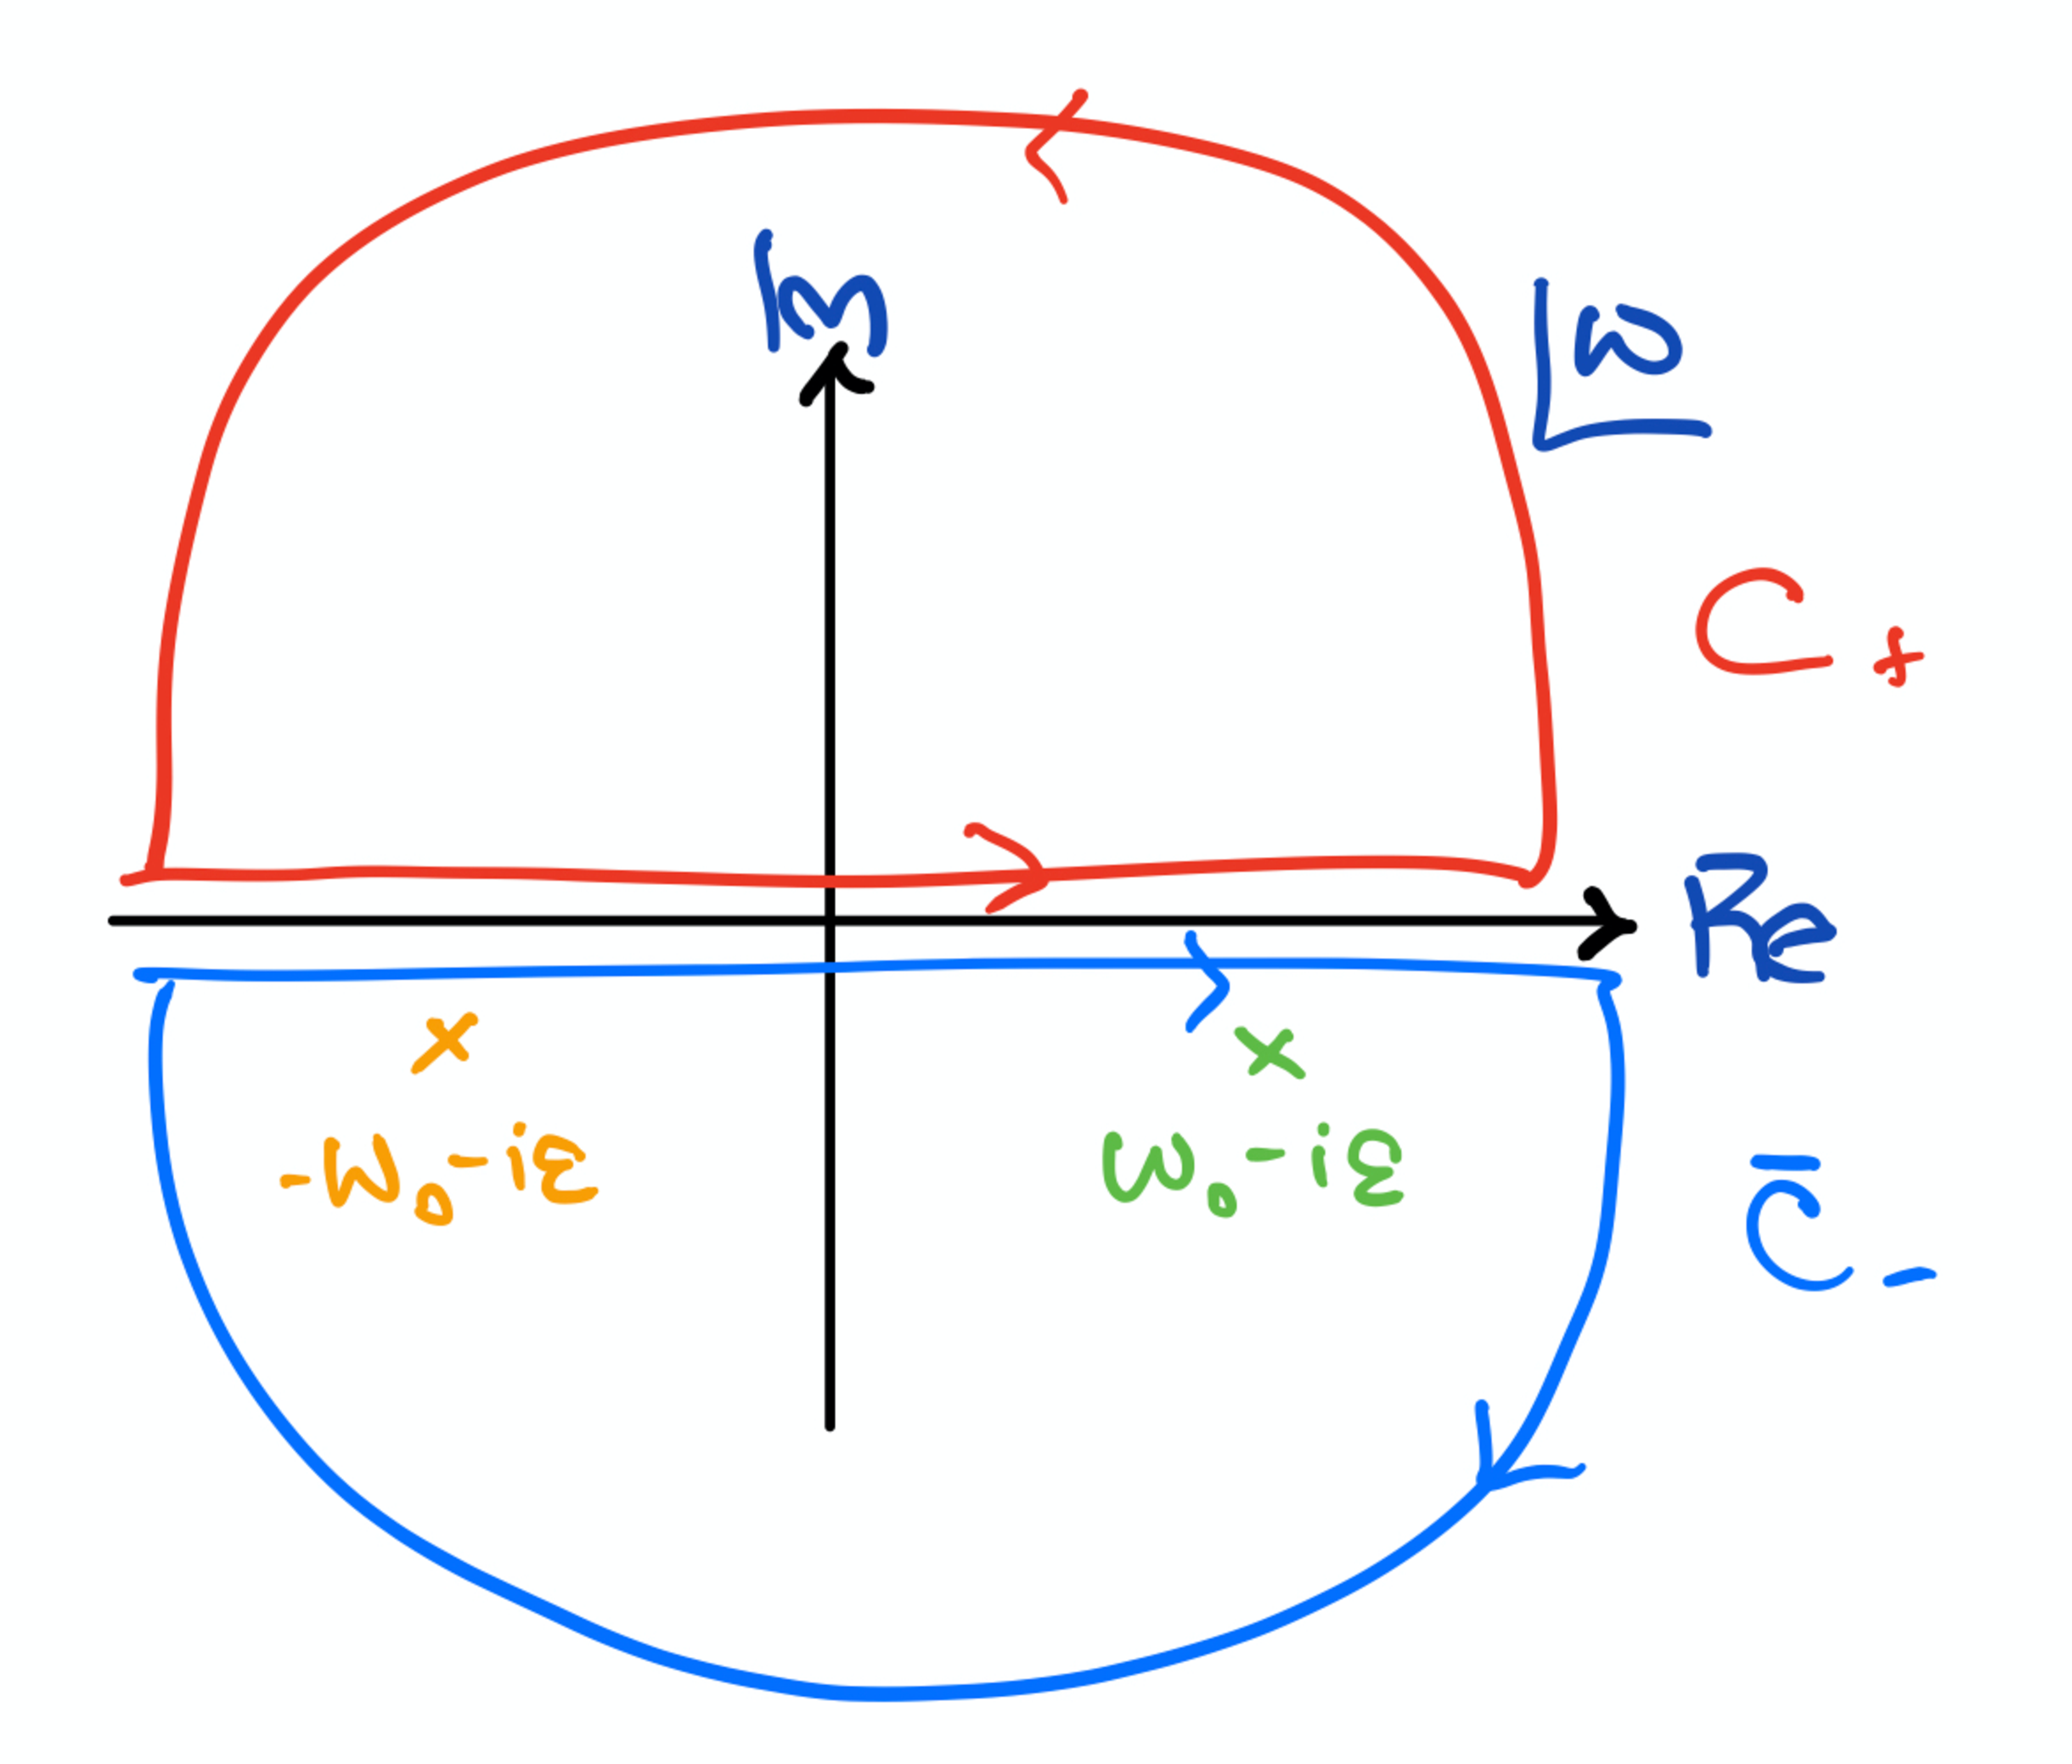
\includegraphics[width=.4\textwidth]{figures/Lec_2017_16_pokedown.pdf}
\end{center}

The integral is exactly the same, except the sign of $\varepsilon$ has changed. 
\begin{exercise}
Pop quiz! Unlike the advanced Green's function where we gave the poles a small positive imaginary part, we have now given the poles a small \textbf{negative} imaginary part. How do we assign the contours $C_+$ and $\bar C_-$ to the cases $t>0$ and $t<0$?
\end{exercise}
Did I fool you? The poles may have moved, but the way that we pick contours does not change: this is fixed by the $e^{-i\omega t}$ factor in the integrand. Thus we \emph{still} have the contour choices in \eqref{eq:t:sign:contour:HO}:
\begin{align}
	t>0 &\to \bar C_{-} 
	&
	t<0 &\to C_+ \ .
\end{align}
What has changed is that now the $\bar C_{-}$ contour encloses poles, whereas the $C_+$ contour encloses no poles. This clearly tells us that the integral over $\omega$ (or its complexificaion $z$) is zero for $t<0$, which means we do not have acausal propagation: 
\begin{align}
	G(t<0) &= 0 \ .
	\label{eq:HO:G:ret:acausal}
\end{align}

What about the causal propagation? Remember that $\bar C_{-}$ has a negative orientation. To keep our signs clear, let's write the integral as negative a contour $C_-$  which has the positive orientation: 
\begin{align}
	\oint_{\bar C_-} = -\oint_{C_-} \ .
\end{align}
We can go ahead and do the integral over $C_-$ using the residue theorem. We're simply re-doing \eqref{eq:HO:G:integral:adv:1} and \eqref{eq:HO:G:integral:adv:2} with $\varepsilon\to -\varepsilon$. Writing $f(z)$ to be the integrand, we have:
\begin{align}
	G(t>0) =& 
	-\frac{1}{2\pi} \oint_{C_-}dz\, f(z)
	\\
	=&
	2\pi i \times -\frac{1}{2\pi} 
	\left(\text{Res}_f(\omega_0) + \text{Res}_f(-\omega_0)\right)
	\\
	=& \frac{1}{\omega_0}\sin(\omega_0 t) \ .
\end{align}
Combining this with \eqref{eq:HO:G:ret:acausal} using the Heaviside $\Theta$-function \eqref{eq:Heaviside:Theta} gives the \textbf{retarded Green's function}:
\begin{align}
	G_\text{ret}(t) &= 
	\frac{1}{\omega_0}
	\sin(\omega_0 t)
	\Theta(t) \ .
	\label{eq:HO:Gret:sin:theta}
\end{align}
\begin{exercise}
Restore $t_0\neq$ in the above equation for the retarded Green's function.
\end{exercise}
By the way, we will often use the word \textbf{propagator} in place of Green's function. This is because the Green's function propagates information from the source to the observation point\footnote{This is especially clear when solving linear differential equations for which the Green's function represents an exact solution. For non-linear problems, one typically resorts to a perturbation expansion. This is what Feynman diagrams are: lines represent propagators, which are Green's functions for the linear part of the dynamical equation. The vertices represent non-linearities which must be treated as a Taylor series about a partition function.}. 


\subsection{Other choices? (Feynman Propagator)}

We've introduced the advanced $G_\text{adv}$ and retarded $G_\text{ret}$ Green's functions. These are both Green's functions for the harmonic oscillator, but for technically different versions of the harmonic oscillator where the differential operator $\mathcal O_t$ has been tweaked to make it slightly complex. We always take the complex part to zero at the end, but we have nudged the poles of the Fourier integrand over a bit and discovered that these have implications on the causality of the Green's function. Clearly the Green's function that we want for most classical applications is the retarded Green's function; this one reflects an effect that happens after the cause.

However, we may as well also explore alternative pole-pushing options. Consider the following mixed prescription:
\begin{center}
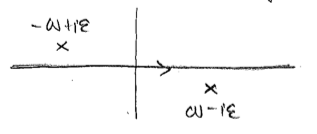
\includegraphics[width=.6\textwidth]{figures/Lec_2017_16_Feynman.png}
\end{center}
Here one pole is pushed up and the other is pushed down. We'll only focus on the case of $+\omega_0$ being pushed into the lower half-plane and $-\omega_0$ being pushed into the upper half-plane. I'll leave it to you to figure out the implications of the converse choice.
\begin{example}
Even before we do any of the work, you should identify why this is strange. The exponential factor of the Fourier integrand determines which contour we select. This, in turn, is based on the sign of $t$ and connects to our notion of causality. By splitting the poles like this, we see that there is a non-zero contribution to \emph{both} causal and acausal propagation. What's even more curious, we no longer get the combination of two complex exponentials that gives a (real) sine. Thus the Green's function is manifestly complex. Curious!
\end{example}
We call this the Feynman propagator, $G_F$, which should make you suspect that this choice is not just some mathematical curiosity but actually has physical significance. The result is:
\begin{align}
	G_F(t>0) &= \frac{i}{2\omega_0} e^{-i\omega_0 t}
	&
	G_F(t<0) &= \frac{-i}{2\omega_0} e^{i\omega_0 t} \ .
	\label{eq:HO:G:Feynman}
\end{align}
\begin{exercise}
Prove \eqref{eq:HO:G:Feynman} using the techniques demonstrated in this section.
\end{exercise}
This Green's function turns out to be the correct choice for quantum field theory. Even if you don't know what quantum field theory is, you can guess from the name that this makes sense:
\begin{enumerate}
\item The `quantum' implies that maybe complex numbers aren't so odd. In fact, the $e^{\pm i\omega_0 t}$ looks a lot like $e^{i\hat H t}$, the time-evolution operator. Indeed, frequencies and energies have the same dimension once you throw in the appropriate factors of $\hbar = 1$.
\item The word `field' implies something like a continuum. Continua are represented by a bunch of nearest-neighbor connected springs---in other words, they are naturally represented as coupled harmonic oscillators\footnote{This fact should be better presented in the standard undergraduate curriculum.}.
\end{enumerate}
What the Feynman propagator/Green's function represents two things, depending on the sign of $t$:
\begin{enumerate}
\item $t>0$: a plane wave moving forward in time with positive energy, $G_F \sim e^{-i\omega t}$. This seems totally fine. The fact that $G_F$ is imaginary is not a big deal, since it now represents something like a wavefunction in quantum mechanics. 
\item $t<0$: a plane wave moving \emph{backward in time} with  with \emph{negative energy}, $G_F \sim e^{-i(-\omega) t}$. This is the suspicious case: note the `double negative' of moving backward in time and having negative energy.
\end{enumerate}
You may know the resolution of the $t<0$ solution since it's a popular story in physics. Dirac found that the solution to the dynamical equation for relativistic electrons contained negative energy electrons moving backward in time. These corresponded to currents of negative charge moving backward in time, which you can hand-wave into understanding as a \emph{positive} charge moving \emph{forward} in time. In other words, rather than describing negative energy electrons moving backward in time, these states correspond to positive-energy positrons moving forward in time. Thus we have a theoretical invitation to the existence of anti-particles\footnote{For those interested in particle or nuclear physics, you may also want to notice that the particle and the anti-particle propagators differ by complex conjugation. This is related to the idea that charges reflect some complex nature of the particles. The geometric description of electrodynamics is a $U(1)$ fibration of spacetime. What this means is that every field is allowed to have a complex phase: the $U(1)$ refers to rephasing symmetry, $z\to e^{i\phi} z$. The other familiar forces of fundamental physics are described by the generalization to what is called $SU(N)$ where an $N$-vector of particles $\Psi^i$ transforms under the $N\times N$ special unitary matrix $U^i_{\phantom i j}=\exp(i\phi^a T^a)^i_{\phantom i j}$ so that $\Psi^i \to U^i_{\phantom i j} \Psi^j$. The matrices $T^a$ are called the `generators' of these $N$-dimensional rephasings. For the case $SU(2)$, the $T^a$ are simply the three Pauli matrices, $\sigma^a$ and the $N$-vectors are essentially two-component spinors. The anti-particles are Hermitian conjugates of the particles $\Psi$.\label{footnote:U1:SUN}}. 


% 2017 - 17

\subsection{Aside: Feynman Green's Function and Convergence of the Path Integral [optional]}

This section is purely `for culture'. We present a qualitative discussion of how one could have anticipated the Feynman propagator from the perspective of the path integral formulation of quantum mechanics. While path integrals are outside the scope of our course, the overall story here is helpful to see how a theory predicts an equation of motion. The Fourier components of the Feynman Green's function are:
\begin{align}
	\tilde G(k) &=
	\frac{-1}{
	\left[k-(\omega_0 -i\varepsilon)\right]
	\left[k-(\omega_0 + i\varepsilon)\right]
	}
	=
	\frac{-1}{
	k^2 - \omega_0^2 + \frac{i}{2} \delta 
	}
	\ ,
	\label{eq:Feynman:G:tilde}
\end{align}
where $2i\epsilon \omega_0 \equiv \delta = \frac{i}{2}\delta$ is just shorthand for a small, positive quantity. This is what we would expect from a Lagrangian:
\begin{align}
	L = \frac{1}{2}\dot x^2 - \frac{1}{2}\left(\omega_0^2 + i \delta\right)x^2 \ .
\end{align}
\begin{exercise}
Check that the equation of motion from this Lagrangian indeed gives a differential operator whose Green's function has Fourier components \eqref{eq:Feynman:G:tilde}.
\end{exercise}
Since the the Lagrangian is related to the action, $S$, by $S=\int dt\, \mathcal L$, one can integrate the $\dot x^2$ term by parts to write:
\begin{align}
	S = -\int dt \, \frac{1}{2}
	x 
	\left[\left(\frac{d}{dt}\right)^2 + \omega_0^2 - i\delta \right]
	x 
	=
	-\int dt \, \frac{1}{2}
	x 
	\left[\mathcal O_\text{HO} - i\delta \right]
	x  \ ,
	\label{eq:HO:S:Feynman:quad}
\end{align}
where $\mathcal O_\text{HO}$ is the original harmonic oscillator differential operator that we started with in \eqref{eq:O:HO}. This shows us that the Feynman prescription for pushing poles around corresponds to adding a small imaginary part to the harmonic oscillator Lagrangian. This is a little weird since the resulting operator is clearly not Hermitian.

If you're familiar with statistical mechanics or quantum field theory, you may know that the fundamental object is neither the Lagrangian nor the action\footnote{... and is definitely not the Hamiltonian; sorry condensed matter folks and Lin-Manuel Miranda fans.}, but actually the path integral, $Z$ which is defined as an integral over all possible functions $x(t)$:
\begin{align}
	Z &= 
	\int \mathcal Dx \, e^{iS[x]}
	= 
	\int \mathcal Dx \, e^{iS_\text{HO}[x] - \frac{\delta}{2} x^2} \ .
\end{align}
Here $\mathcal Dx$ is just the measure of the path integral. For discretized space, it corresponds to $\mathcal Dx\sim dx(t_0)\,dx(t_1)\, dx(t_2)\cdots$. The harmonic oscillator action $S_\text{HO}$ is real and thus $e^{iS_\text{HO}}$ oscillates and the path integral doesn't converge. By adding the $- \frac{\delta}{2} x^2$ term to the action we are imposing a small perturbation that forces the integrand to converge for very large values of $x(t)$. With this factor the path integral is well defined. If we approached the harmonic oscillator assuming that path integral is sufficiently convergent\footnote{Physically this is saying that these extreme path configurations should not contribute since the path that minimizes the action should be far away from these cases; so we're just helping the theory focus on the part of the path integral that matters.} and plugging in some factor to force this convergence, then we can run this argument backward and `deduce' the Feynman prescription for the Green's function.

If everything in this subsection is a bit boring, then here's what you should know. This discussion gives us a hint of where all of our physical differential equations come from. The equations of motion that define a theory come from a variational principle with respect to some action. 
\begin{exercise}
[optional] What is the action (Lagrangian, Hamiltonian, whatever...) that yields Maxwell's equations? Note that curiously, you only get half of Maxwell's equations from an action principle. The other half comes from the geometry alluded to in Footnote~\ref{footnote:U1:SUN} and the ideas in Section~\ref{sec:stokes:theorem:aside}. For a discussion by a well-known \acro{UCR} mathematical physicist, see \emph{Gauge Fields, Knots And Gravity} by Prof.~John Baez.
\end{exercise}
We then recall that our actions (Lagrangians, Hamiltonians, ...) tend to be \emph{local} function(al)s, so it makes sense that they can be written as a derivative expansion. The actions depend on particles/fields, say\footnote{I'm deliberately changing notation from $x(t)\to q(t)$. This is important because we will eventually want to treat $x$ and $t$ as spacetime coordinates rather than $x(t)$ as `the position of \emph{the} particle at time $t$.' This unfortunately notational confusion tends to be one of the conceptual hurdles in field theory.} $q(t)$. If we write out the leading terms of the action with respect to $q(t)$ you get something like
\begin{align}
	S[q] &= \int dt \, (\text{const.}) + \mathcal O_1 q(t) + \mathcal O_2 q^2(t) + \mathcal O_3 q^2(t) + \cdots
\end{align}
where the $\mathcal O_i$ are differential operators. We can ignore the constant. Usually the $\mathcal O_1$ term doesn't show up, so let's ignore that too; you can remove it by redefining the particle\footnote{The linear term tells you that you're probably not defining the `zero' of your field sensibly. Amusingly, this is closely related to the Higgs phenomenon that gives known fundamental particles most of their mass.}. The $\mathcal O_2 q^2$ term can be integrated by parts. The details of the integration by parts depend on the details of the derivatives in $\mathcal O_2$, but one can write typically write this term as
\begin{align}
	\mathcal O_2 q^2(t) &\equiv - q(t) \mathcal O_\text{quad} q(t) \ ,
\end{align}
which is in the form that we used in \eqref{eq:HO:S:Feynman:quad}. When we derive the equation of motion by varying the action, we end up with
\begin{align}
	-\mathcal O_\text{quad} q(t) = 0 \ ,
\end{align}
where I'm probably assuming that $\mathcal O_\text{quad}$ is Hermitian if we want to be technical. The main observation here is that this is a \emph{linear} differential equation. Linear differential equations in physics come from the quadratic pieces of actions. Since we argued that the linear piece is usually not there and we know that the constant piece corresponds to a shift in the vacuum energy (that's \emph{usually} not physical\footnote{Damn you, dark energy.}), then this quadratic piece of the action is the \emph{lowest order} contribution to the action in an expansion of the particle $q(t)$ with respect to the vacuum ($q(t)=0$). The higher-order terms correspond to differential equations that are \emph{not} linear since the variation of that term contains $q^2(t)$. So yes, even though the mathematical structures here are a bit more fancy, let us state out loud that all of our main differential equations in physics basically boil down to taking the leading term in a Taylor expansion. Typical for physicists, eh?

% 2017 - 17: skipping Kramers Kronig for now

% 2017 - 18: skipping Kramers Kronig for now

\subsection{Example: The Damped Harmonic Oscillator}
 
 At this point we are happy that the physical solution to the classical harmonic oscillator is the retarded Green's function, $G_\text{ret}(t)$. There is an unphysical solution, the advanced Green's function, $G_\text{adv}(t)$ that reflects a mathematical symmetry of the theory (time-reversal invariance) but is otherwise not of physical interest. Finally, there is a solution that makes sense for quantum physics, the Feynman Green's function, $G_\text{F}(t)$, which is complex but reflects the existence of anti-particles. Each of the above cases came from \emph{almost} the same harmonic oscillator differential operator, $\mathcal O$, except the operators were slightly deformed so that its poles were off of the real line in the complex momentum plane. We took the limit where this deformation goes to zero, but not until after we've exploited those deformations to do the Fourier integral using the residue theorem. We came to appreciate that the infinitesimal nudge in the imaginary direction was telling us something about the causality of the harmonic oscillator.

 We can understand the nature of this imaginary push by looking at the \emph{damped harmonic oscillator}. The dynamical equation for the damped harmonic oscillator is
 \begin{align}
 	\mathcal O_\text{DHO} x(t) = \ddot{x}(t) + 2\gamma\dot x(t) + \omega_0^2 x(t) = F(t) \ ,
 \end{align}
 where $\gamma$ is the \textbf{damping coefficient} and $F(t)$ is a driving force.
 \begin{exercise}
 What are the dimensions of the damping coefficient, $\gamma$?
 \end{exercise}
 
 \paragraph{Back of the envelope version.}
 Before doing anything quantitative, we can guess the behavior. A non-zero $\gamma$ suppresses the response $x(t)$ to the source $F(t)$. Unlike an idealized instrument, a guitar string has non-zero damping and the vibrations get smaller the longer you wait after plucking it. If we imagine a plane wave\footnote{I keep calling $e^{-i\omega t}$ a plane wave because I'm thinking of the generalization to spacetime. For now there are no transverse directions, so of course $e^{-i\omega t}$ is really just a wave.} $x(t)\sim e^{-i\omega t}$ and ask what this wave looks like far away from the source, $F(t)\to 0$, then the differential equation reads:
 \begin{align}
 	-\left(\omega^2 +2i\gamma \omega - \omega_0^2\right)e^{-i\omega t} &= 0 \ .
 \end{align}
 The solution for the plane wave's frequency $\omega$ is
 \begin{align}
 	\omega = \omega_R - i\Gamma \ , \label{eq:DHO:back:envelope:poles}
 \end{align}
 where for $\gamma^2 \ll \omega_0^2$, $\omega_R \approx \omega_0$ is the frequency.  Plugging $\omega$ back into our plane wave gives
 \begin{align}
 	x(t) = e^{-i\omega_R t}e^{-\gamma t} \ .
 \end{align}
 The first factor is the usual plane wave. We recognize the $\exp(-\gamma t)$ as an exponential suppression that causes the plane wave to get rapidly smaller for times larger than $1/\gamma$. There are a few lessons:
 \begin{enumerate}
 \item In \eqref{eq:DHO:back:envelope:poles} we have implicitly but decisively bought into the idea of a complex frequency. The interpretation of this complex frequency is that the real part is the usual oscillation and the imaginary part corresponds to damping.

 \item The solution \eqref{eq:DHO:back:envelope:poles} corresponds to finding the poles of the Fourier integrand; recall, for example, \eqref{eq:G:HO:Fourier:equation:integrals}. So damping has something to do with the imaginary part of the poles in the complex plane.

 \item Because the position of the pole in the imaginary direction is related to the \emph{causality} of the theory, we have now connected `damping' to causality in a round-about way.

 \item When we derived the retarded Green's function $G_\text{ret}(t)$ that describes the classical, ideal harmonic oscillator, we took $i\varepsilon\to 0$. For the damped harmonic oscillator the corresponding value is $i\gamma$, which we keep finite\footnote{Here's a funny bit of linguistics in our discipline. Any physical quantity is naturally not-infinite, so it seems silly when physicists make a point to call something `finite.' You would think that this is in contrast to that quantity being infinite. In fact, when physicists say \emph{finite} what they really mean is \emph{not zero}, which is quite different from `not infinite.'}; it has some physical significance after all.

 \item The exponential notation for the Fourier transform made all of this very easy: we just let $\omega$ be complex in $e^{-i\omega t}$ and we are able to capture the physics of oscillations and damping. If we had used trigonometric functions then we'd have a bunch of $\sinh$ or $\cosh$ floating around and the convergence would not be so clear.
 \end{enumerate}
 
 \paragraph{More carefully.} Let's go through the steps to derive the Green's function for the damped harmonic oscillator properly. The Green's function equation is
 \begin{align}
 	\left[
 	\left(\frac{d}{dt}\right)^2
 	+ 2\gamma \frac{d}{dt}
 	+ \omega_0^2
 	\right]
 	G(t)
 	&=
 	\delta(t) \ ,
 \end{align}
 where we've again set $t_0 = 0$. It is easy at this stage to restore\footnote{There is a theorem that $G(t,t')$ only depends on $|t-t'|$ under reasonable assumptions. You should be able to argue this on physical grounds.} $t_0$ by taking $t\to (t-t_0)$. Plugging in the Fourier representations for the $t$-dependence,
 \begin{align}
 	G(t) &= \int \dbar \omega \, e^{-i\omega t}\tilde G(\omega)
 	&
 	\delta(t) &= \int \dbar \omega e^{-i\omega t} \ ,
 \end{align}
 then gives:
 \begin{align}
 	\tilde G(\omega) &=
 	\frac{-1}{\omega^2+2i\gamma\omega -\omega_0^2} \ .
 \end{align}
 The poles occur at 
 \begin{align}
 	\omega_\pm &= \frac{-2i\gamma \pm \sqrt{-4\gamma + 4\omega_{0^2}}}{2}
 	= \pm \sqrt{\omega_0^2 - \gamma^2} - i \gamma \equiv \pm \omega_R - i\gamma\ .
 	\label{eq:DHO:poles}
 \end{align}
 \begin{example}
 The poles in \eqref{eq:DHO:poles} have a real part as long as $\omega_0^2 > \gamma^2$. What does it mean when $\omega_0^2 < \gamma^2$? This is the observation that the damping is stronger than the characteristic oscillation frequency, $\omega_0$. Thus the system is properly describe by an exponentially suppression because it never has a chance to oscillate.\footnote{This is one of the magical things about $B$ mesons. $B$ mesons are really nice systems whose characteristic oscillation frequency (between $B$ and anti-$B$ mesons) and characteristic decay width are roughly of the same order of magnitude. When we produce $B$ mesons at, say, the LHCb experiment, we get to observe the decays (imaginary part) of these mesons after $\sim 1$ oscillation which gives a powerful tool for studying matter--anti-matter asymmetry.\label{footnote:B:meson}}
 \end{example}
 Assuming $\omega_0^2 > \gamma^2$, then we may identify $\omega_R = +\sqrt{\omega_0^2 - \gamma^2}$ and the poles may be written as $\pm \omega_R - i\gamma$. This looks a \emph{just} like the pole prescription for the retarded Green's function of the ideal harmonic oscillator with $\omega_0\to \omega_R$ and $i\varepsilon\to i\gamma$. In fact, we can just follow all of the same steps that we did for the retarded Green's function:
 \begin{enumerate}
 \item The poles are in the lower half-plane of $\omega$. This means that the propagator is automatically causal (it's the retarded, not the advanced Green's function).
 \item The exponential factor $e^{-i\omega t}$ in the Fourier integral determines the convergence of the integrand and hence how we complete the contour. For $t>0$ we close the contour on the lower half-plane and pick up these poles in the residue theorem. For $t<0$ we close the contour on the upper half-plane; since there are no poles here, the Fourier integral vanishes.
 \item We end up with our own version of \eqref{eq:HO:Gret:sin:theta} with $\omega_0\to\omega_R$ except we need to account for the finite $\gamma$. 
 \end{enumerate}
 The only substantial difference between the damped harmonic oscillator and the ordinary harmonic oscillator is that $\omega_\pm$ contains a non-negligible imaginary part. The contour integral takes the form:
 \begin{align}
 	\oint_C dz \,
 	\frac{-e^{-izt}}{
 	\left(z-\omega_+\right)
 	\left(z-\omega_-\right)
 	}
 	=&
 	\phantom+ 
 	2\pi i\left(\text{Res}_f\omega_+ + \text{Res}_f\omega_-\right)
 	\\
 	=&
 	-2\pi i\left[
 	\frac{e^{i\omega_+t}}{\omega_+-\omega_-}
 	+
 	\frac{e^{i\omega_-t}}{\omega_--\omega_+}
 	\right]
 	\\
 	=&
 	-2\pi i
 	\frac{e^{i\omega_+t} - e^{i\omega_-t}}{\omega_+-\omega_-}
 	\\
 	=&
 	-2\pi i \frac{e^{-i\gamma t}}{2\omega_R}
 	\left(e^{i\omega_Rt} - e^{-i\omega_Rt}\right)
 	\\
 	=&
 	\pi \frac{e^{-i\gamma t}}{2\omega_R}
 	\sin(\omega t)
 	 \ .
 \end{align}
 Plugging this into the full solution---which involves keeping track of which contour integral is non-zero and where the factors of $2\pi$ belong---we find:
 \begin{align}
 	G(t) = \frac{e^{-\gamma t}}{\sqrt{\omega_0-\gamma^2}} \sin\left(\sqrt{\omega_0^2-\gamma^2} t\right) \Theta(t) \ .
 	\label{eq:DHO:G:sin:theta}
 \end{align} 
 \begin{exercise}
Compare and contrast \eqref{eq:DHO:G:sin:theta} to \eqref{eq:HO:Gret:sin:theta}. Why is the general form the same? How do you explain the differences? What is the behavior for $\omega \gg \gamma$, $\omega \ll \gamma$? What does it look like if you restored $t_0$?
 \end{exercise}
 The key observation that we have from this discussion is that the choice of pushing the poles into the lower half plane---which we found was critical for a causal Green's function---is actually physically motivated. Any \emph{physical} oscillating system actually has some small amount of friction (or the appropriate generalization) that causes it to not only oscillate, but also decay. 
 \begin{exercise}
 In quantum mechanics the time evolution operator is $e^{i\hat H t}$. Maybe there's a minus sign in there, I don't remember and I don't really care. It is important that this operator is unitary, or else probabilities are not preserved in time. However, there are plenty of physical systems (say, the $B$ meson in footnote~\ref{footnote:B:meson}) that \emph{are} described my non-Hermitian Hamiltonians, i.e.~non-unitary time evolution operators. Reason tells us that the form of the time-evolution operator should be $e^{i\hat H t}e^{-\gamma t}$, since probabilities less than one make more sense than probabilities bigger than one. What is the physical interpretation of this non-unitary time evolution? Hint: this has to do with the notion that our theory (our Hamiltonian) models something in nature, but it not model \emph{all} of the relevant pieces nature for a given problem.
 \end{exercise}
 At this point in my note I have the following written:
 \begin{quote}
 \emph{I took 7 weeks of physics 231 and all I have is this one stupid Green's function.}
 \end{quote}
 
 
 